\subsubsection{pr08}
\label{subsubsec:pr08}
The obtained results were the following:
{
\renewcommand{\arraystretch}{2}
\begin{longtable}[h]{| c | c | c | c | c |}
    \hline
    \textbf{Failures} & \multicolumn{3}{c}{\textbf{Time limit}} & \\
    \hline
    \textbf{Search strategy} & \textbf{\textit{30 sec}} & \textbf{\textit{1 min}} & \textbf{\textit{2 min}} & \textbf{\textit{5 min}} \\
    \hline
    \endhead
    default search                                         & 6.524 & 12.845 &  27.623 & 132.548 \\
    \hline
    domWdeg, random                                        &  468 & 15.198 &  43.892 & 145.073 \\
    \hline
    domWdeg, random, Luby restart L=250                    &  576 &  2.085 &   5.847 &  41.298 \\
    \hline
    \textit{domWdeg, random, Luby restart L=250, LNS 85\%} &   84 &    87 &     94 &    977 \\
    \hline
    domWdeg, random, Luby restart L=250, LNS 15\%          & 1.604 &  5.620 &  17.275 &  75.419 \\
    \hline
    first fail, min                                        & 2.117 & 10.555 &  22.769 &  70.329 \\
    \hline
\end{longtable}
}
\begin{figure}[H]
    \centering
    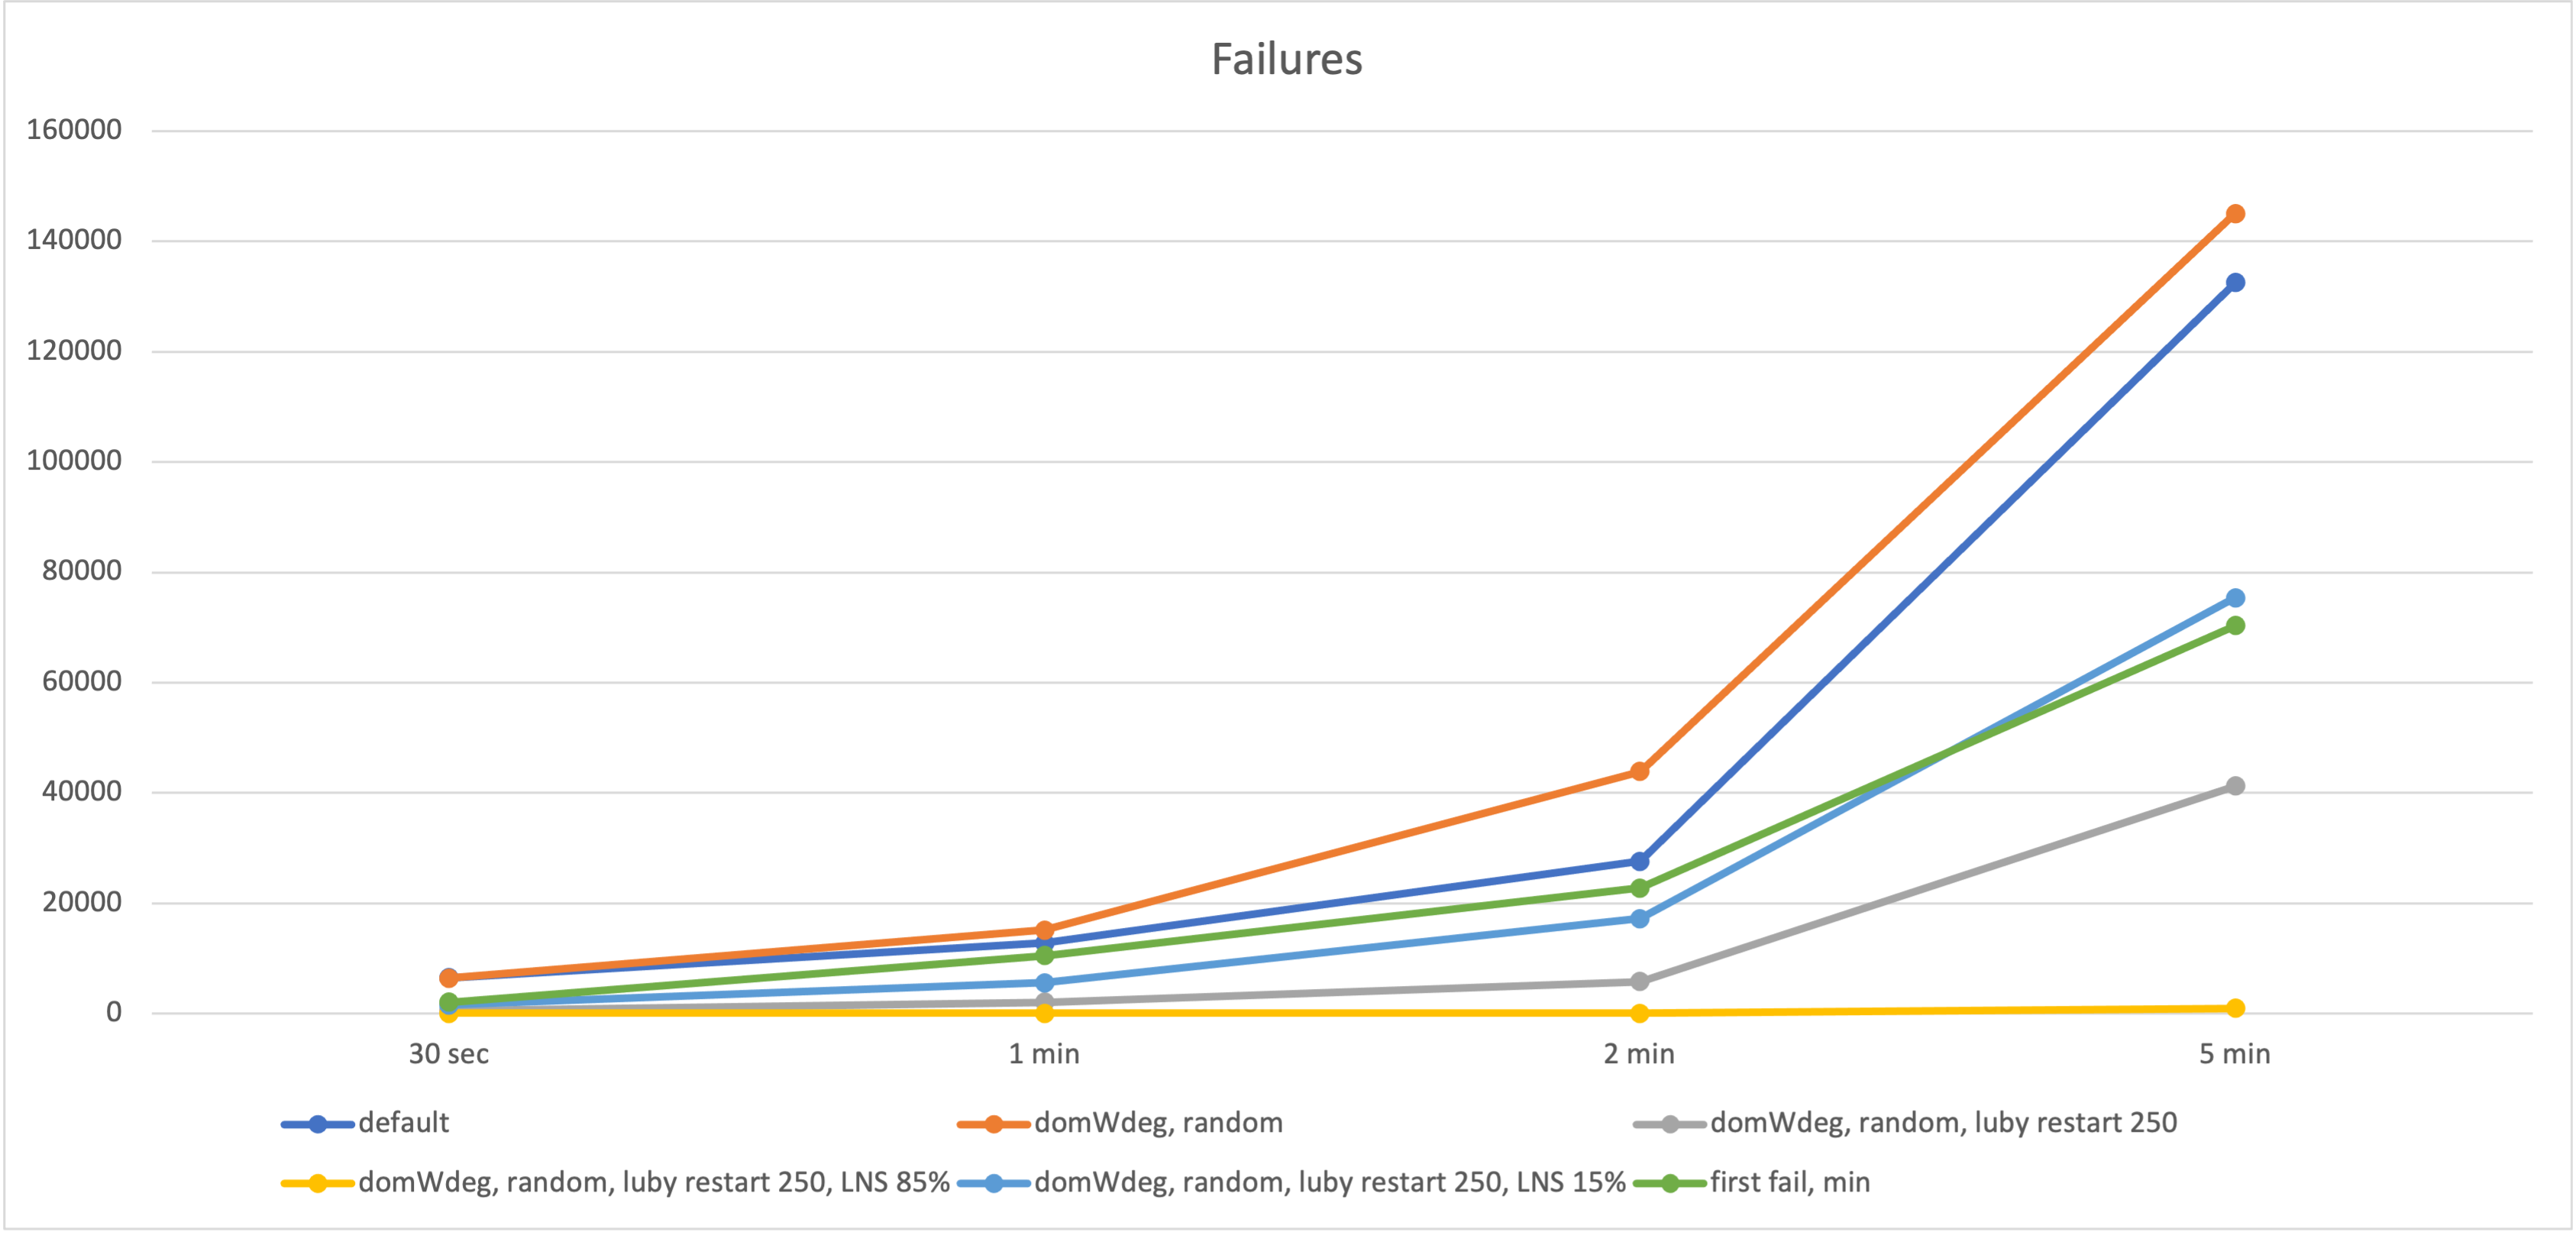
\includegraphics[width=0.8\columnwidth]{../graphs/pr08-failures.png}
    \caption{Failures graph for \textbf{pr08}.}
\end{figure}

{
\renewcommand{\arraystretch}{2}
\begin{longtable}[h]{| c | c | c | c | c |}
    \hline
    \textbf{Objective function} & \multicolumn{3}{c}{\textbf{Time limit}} & \\
    \hline
    \textbf{Search strategy} & \textbf{\textit{30 sec}} & \textbf{\textit{1 min}} & \textbf{\textit{2 min}} & \textbf{\textit{5 min}} \\
    \hline
    \endhead
    default search                                         & 103.320.040 & 102.806.670 & 101.803.020 & 100.469.070 \\
    \hline
    domWdeg, random                                        & 106.998.800 & 106.729.450 & 105.998.510 & 105.539.480 \\
    \hline
    domWdeg, random, Luby restart L=250                    & 109.402.200 & 107.270.420 & 106.454.570 &  98.994.160 \\
    \hline
    \textit{domWdeg, random, Luby restart L=250, LNS 85\%} & 109.464.530 & 106.856.800 & 100.704.630 &  92.217.490 \\
    \hline
    domWdeg, random, Luby restart L=250, LNS 15\%          & 109.622.130 & 103.355.070 & 102.866.190 &  99.720.920 \\
    \hline
    first fail, min                                        & 102.695.400 & 102.286.360 & 101.871.420 & 100.805.580 \\
    \hline
\end{longtable}
}
\begin{figure}[H]
    \centering
    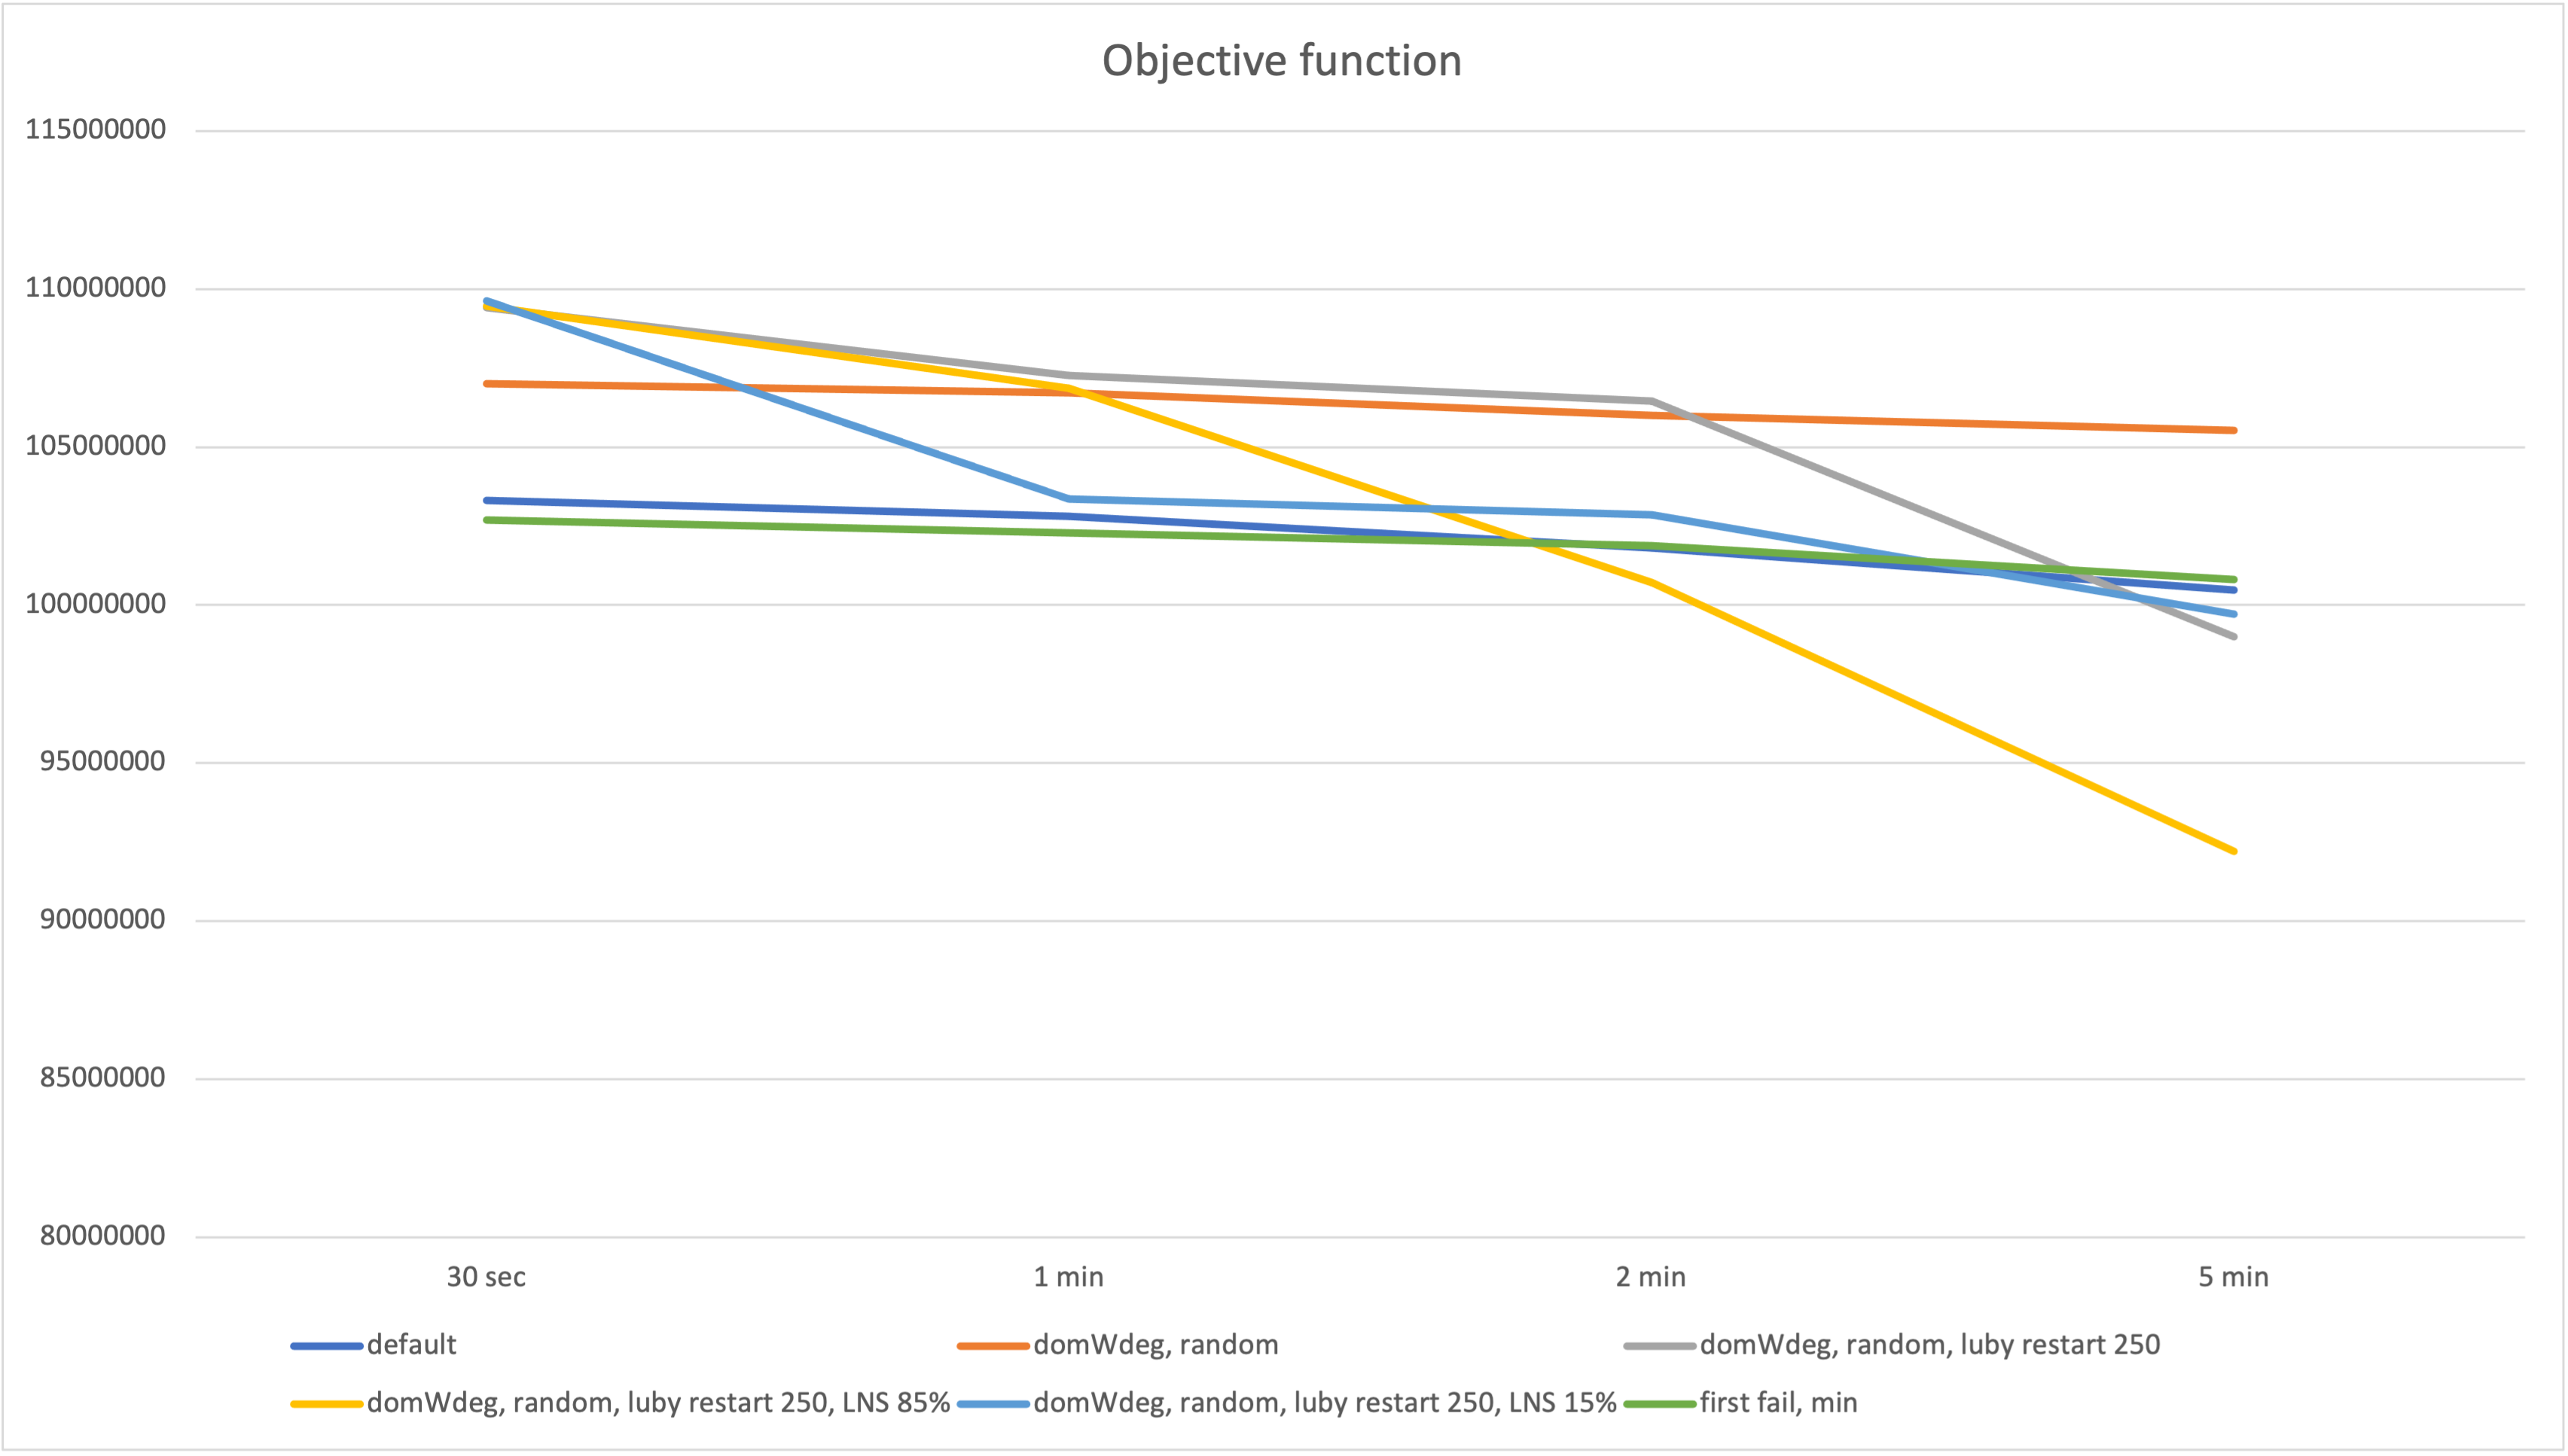
\includegraphics[width=0.8\columnwidth]{../graphs/pr08-objf.png}
    \caption{Objective functions graph for \textbf{pr08}.}
\end{figure}

{
\renewcommand{\arraystretch}{2}
\begin{longtable}[h]{| c | c | c | c |}
    \hline
    \textbf{Weights} & \textbf{Objective function} & \textbf{Total distance} & \textbf{Used vehicles} \\
    \hline
    \endhead
    $\alpha = 10, \beta = 0$ & 86.769.510 &  8.676.951 & 20 \\
    \hline
    $\alpha = 7, \beta = 3$  & 61.093.667 &  8.727.659 & 18 \\
    \hline
    $\alpha = 5, \beta = 5$  & 43.946.875 &  8.789.357 & 18 \\
    \hline
    $\alpha = 3, \beta = 7$  & 25.887.777 &  8.629.224 & 15 \\
    \hline
    $\alpha = 0, \beta = 10$ &        120 & 11.137.732 & 12 \\
    \hline
\end{longtable}
}
\begin{figure}[H]
    \centering
    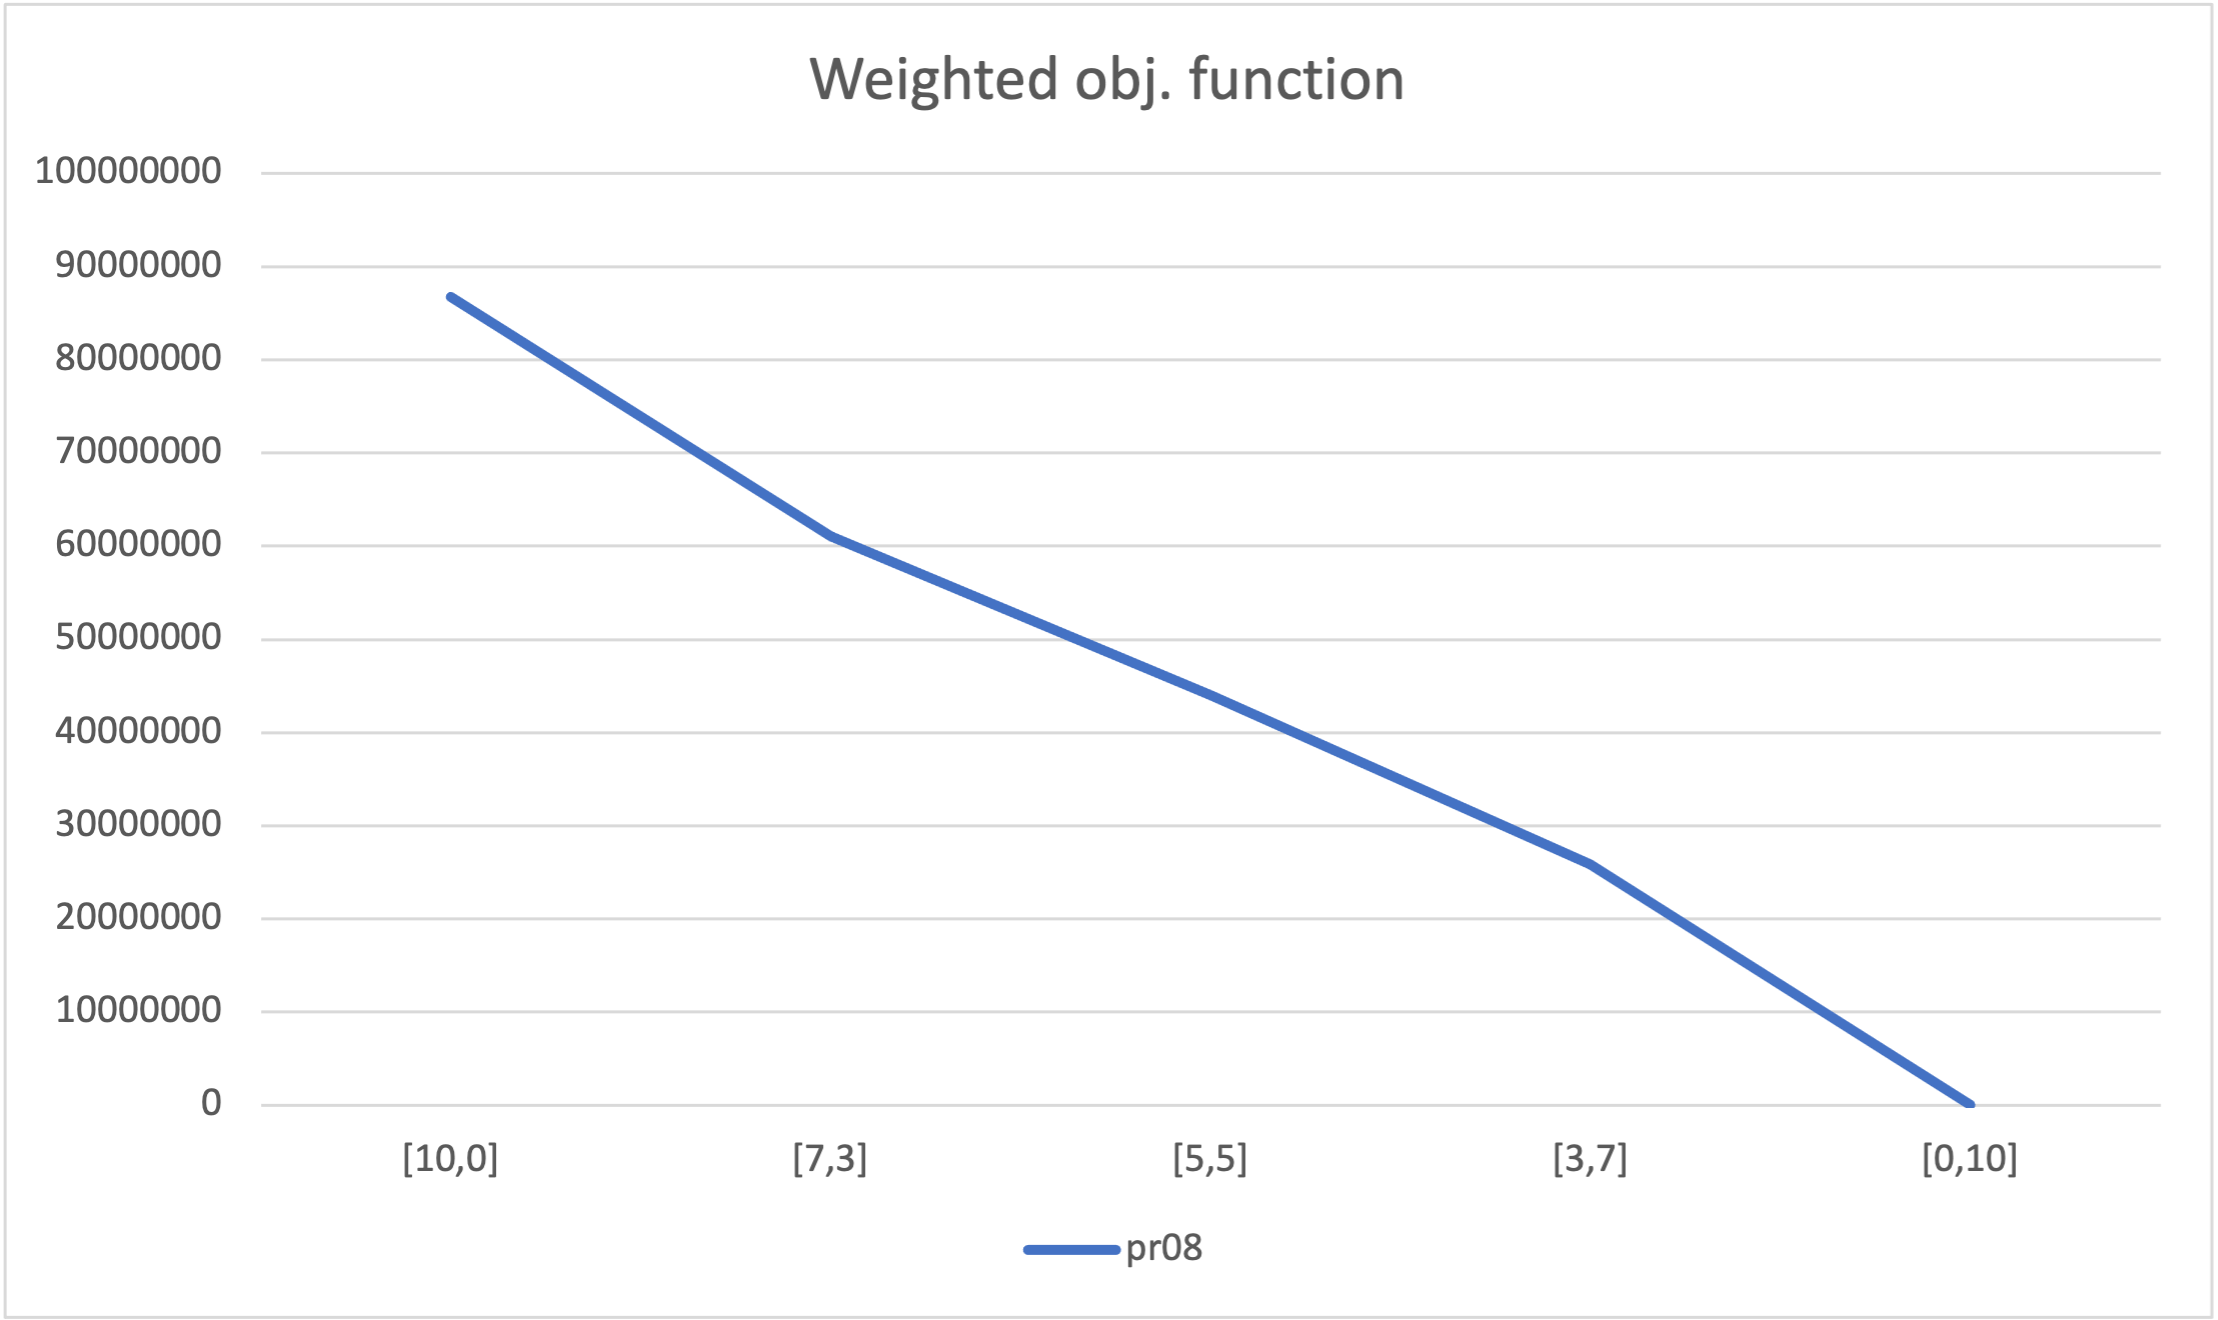
\includegraphics[height=0.25\textheight]{../graphs/pr08-wobjf.png}
    \caption{Weighted objective functions graph for \textbf{pr08}.}
\end{figure}

\begin{figure}[H]
    \centering
    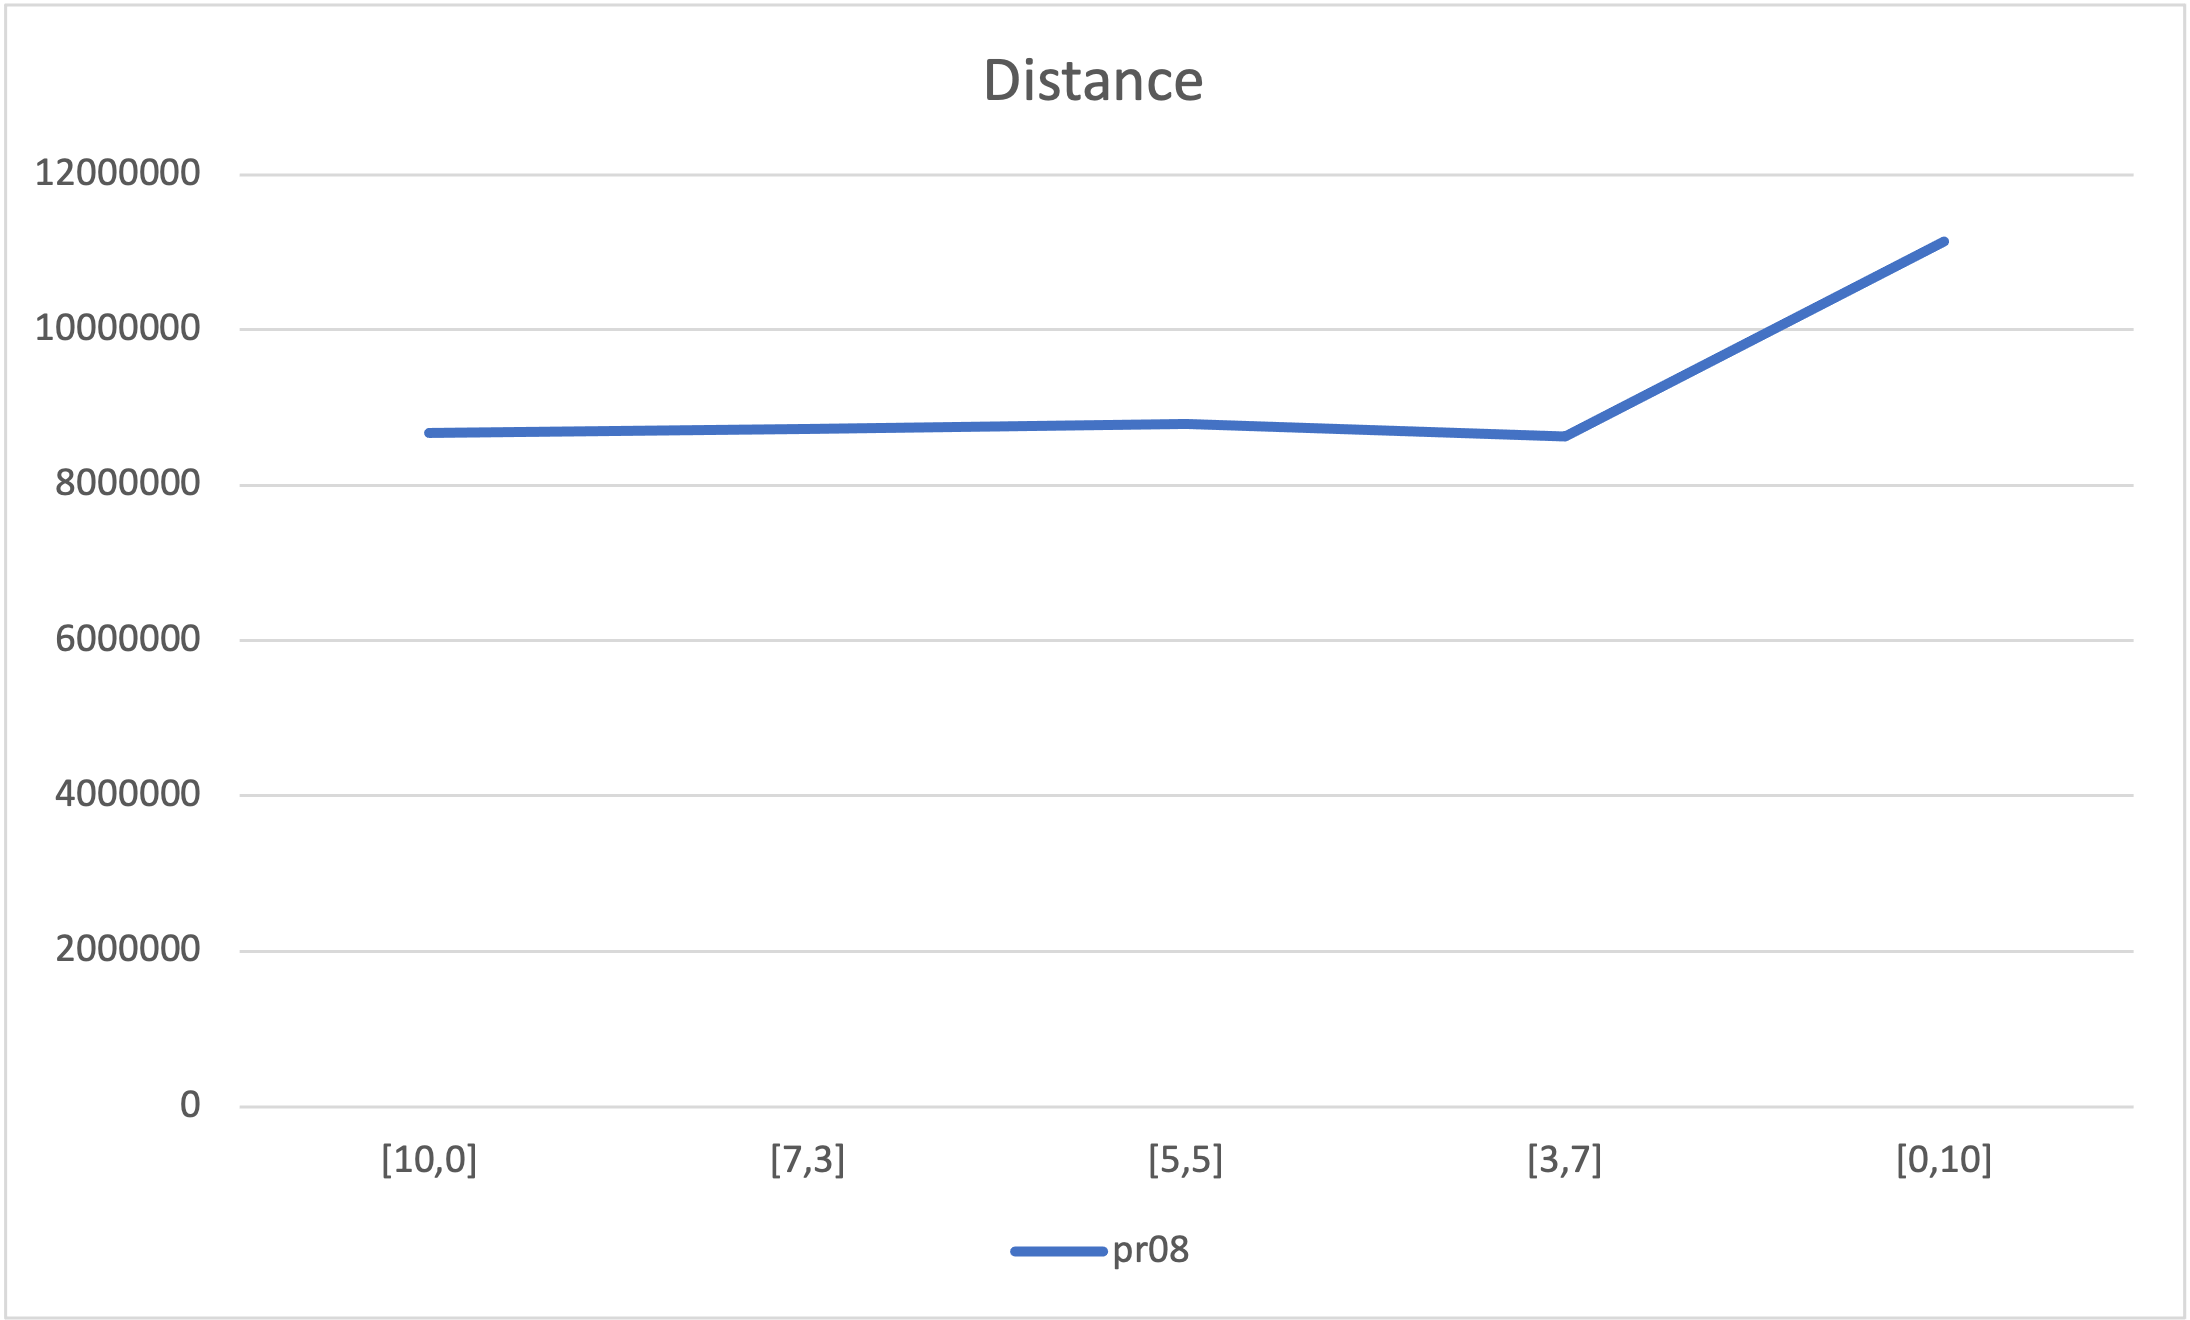
\includegraphics[height=0.25\textheight]{../graphs/pr08-distance.png}
    \caption{Distances graph for \textbf{pr08}.}
\end{figure}

\begin{figure}[H]
    \centering
    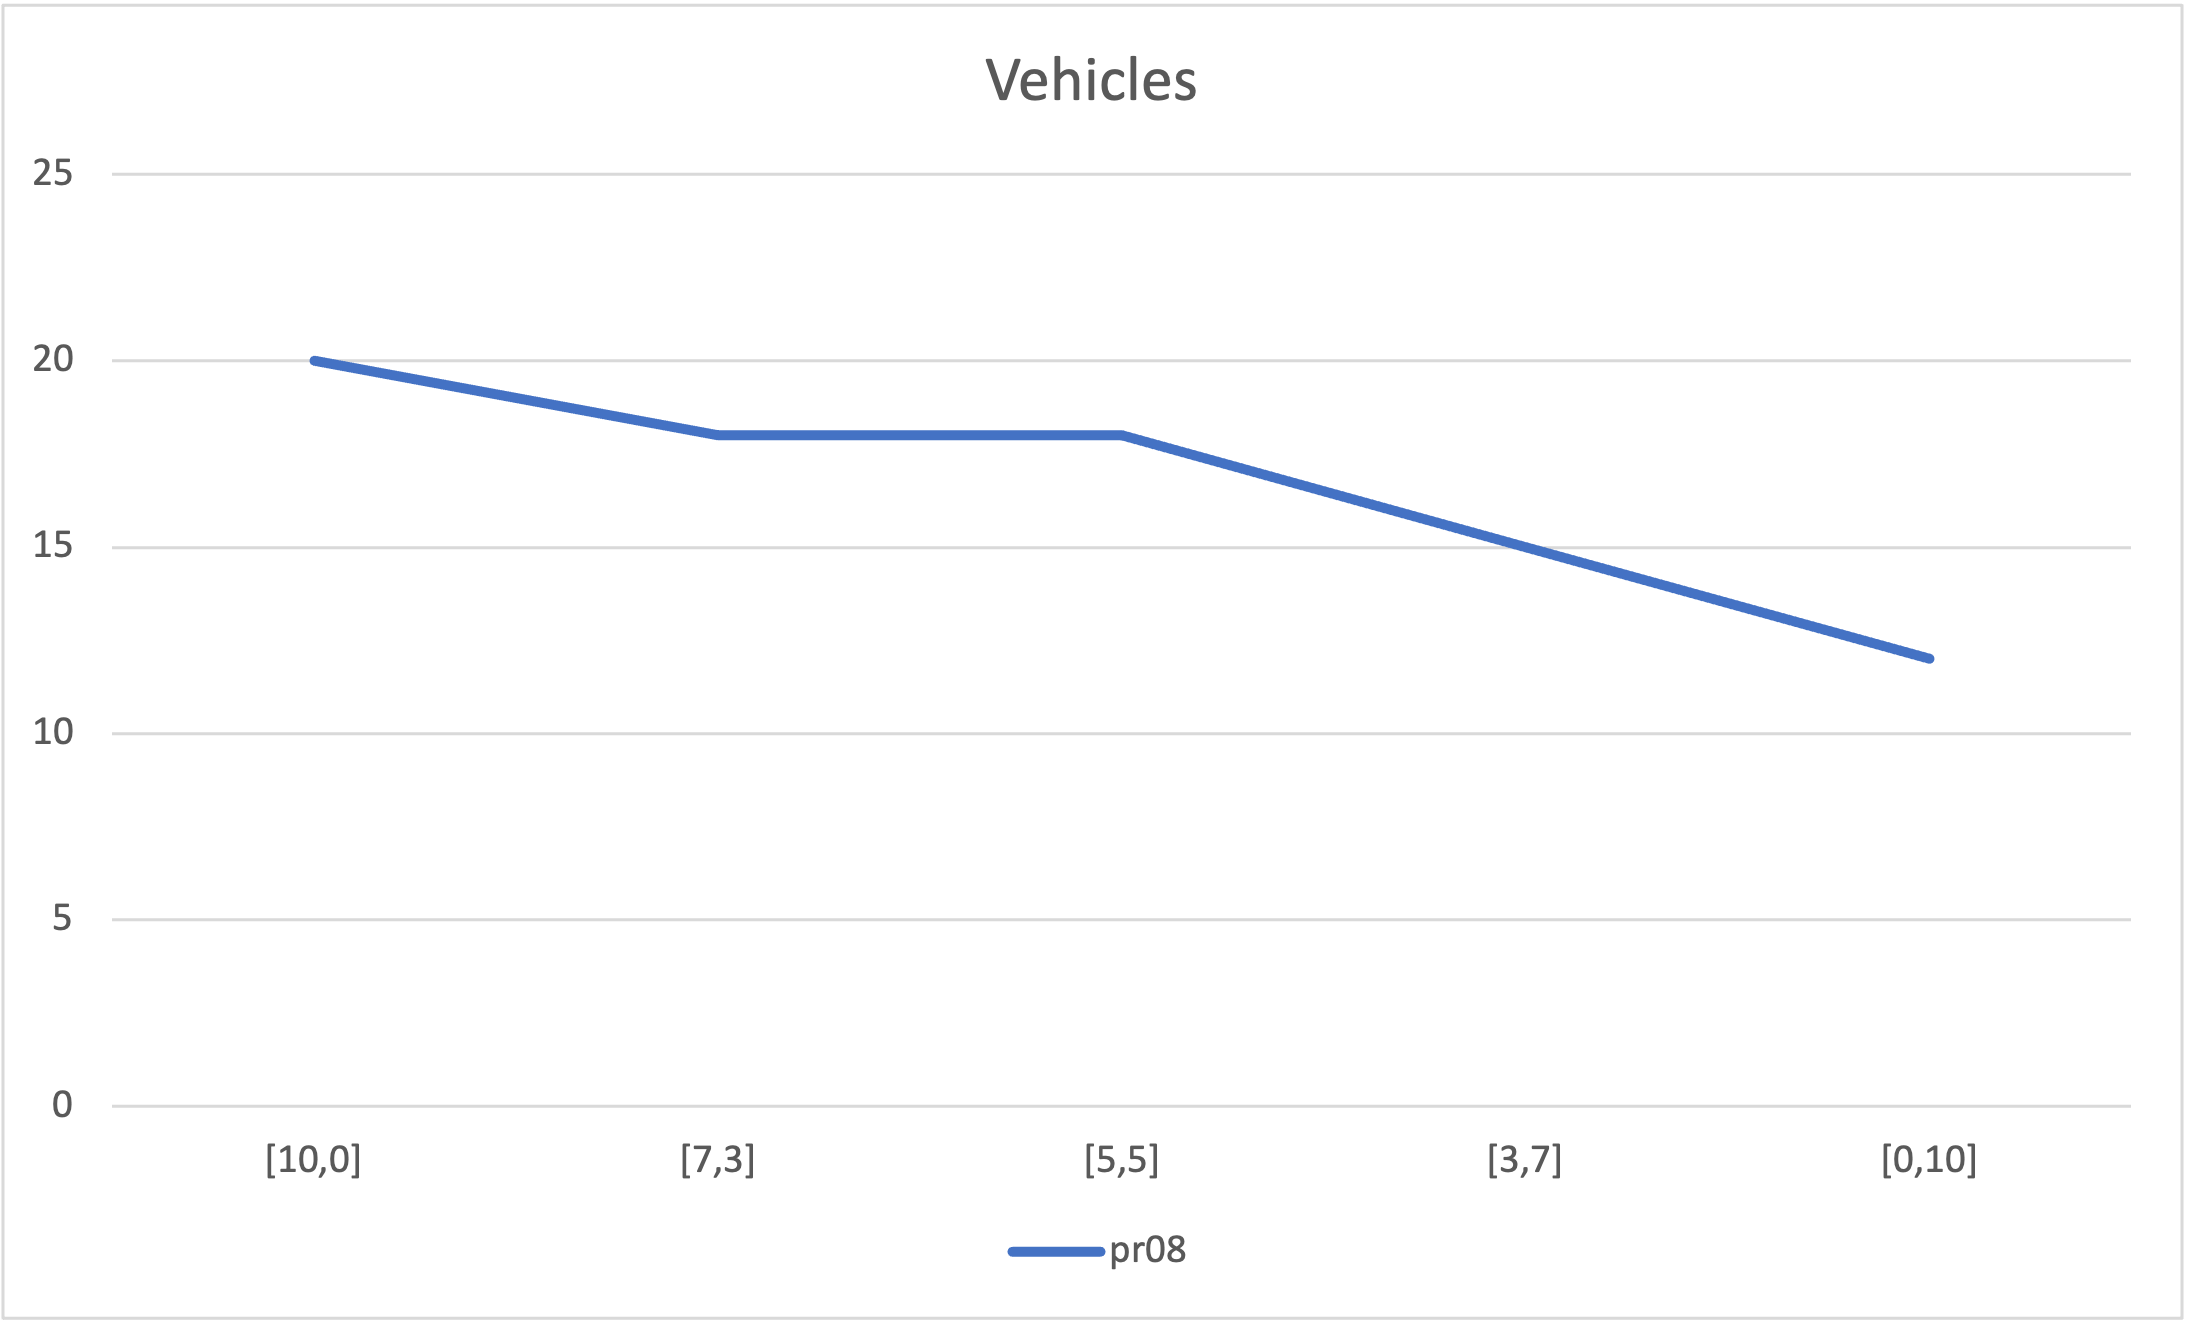
\includegraphics[height=0.25\textheight]{../graphs/pr08-vehicles.png}
    \caption{Used vehicles graph for \textbf{pr08}.}
\end{figure}

\newpage
